\documentclass[twocolumn]{article}

\usepackage[backend=biber]{biblatex}
\usepackage[T1]{fontenc}
\usepackage{hyperref}
\usepackage{booktabs}
\usepackage{subcaption}
\usepackage{tikz}
\usepackage{expl3}
\usepackage{amsmath}
\usepackage{amssymb}
\usepackage{todonotes}

% Layout
\setuptodonotes{inline}


% Math declarations
\DeclareMathAlphabet\mathbfcal{OMS}{cmsy}{b}{n}
\newcommand{\ten}[1]{\underline{\mathbf{#1}}} % tensor
\newcommand{\mat}[1]{\mathbf{#1}} % matrix
\renewcommand{\vec}[1]{\mathbf{#1}} % matrix
\newcommand{\mpr}[2]{\times_{#2} {#1}_{#2}} % mode product
\newcommand{\mmpr}[1]{\times\{#1\}} % multi-mode product
\newcommand{\mmprs}[2]{\times_{-#2}\{#1\}} % multi-mode product
\newcommand{\ev}[2]{\text{E}\left[#1\right]_{#2}}
\DeclareMathOperator*{\argmax}{arg\,max}
\DeclareMathOperator*{\argmin}{arg\,min}
\newtheorem{theorem}{Theorem}

% Includes
\addbibresource{references.bib}
\newcommand{\Width}{2}
\newcommand{\Height}{2}
\newcommand{\Depth}{2}
\newcommand{\TensorThree}[7]{
	\renewcommand{\Width}{#5}
	\renewcommand{\Height}{#6}
	\renewcommand{\Depth}{#7}
	\coordinate (O) at (0,0,0);
	\coordinate (A) at (0,\Height,0);
	\coordinate (B) at (0,\Height,\Depth);
	\coordinate (C) at (0,0,\Depth);
	\coordinate (D) at (\Width,0,0);
	\coordinate (E) at (\Width,\Height,0);
	\coordinate (F) at (\Width,\Height,\Depth);
	\coordinate (G) at (\Width,0,\Depth);
	\node at (\fpeval{0.5*#5},\fpeval{0.5*#6},\Depth) {#1};
	\draw[densely dotted] (O) -- (A);
	\draw (O) -- (C)node[midway,xshift=-.5em, yshift=.5em] {#4};
	\draw (O) -- (D);
	\draw (F) -- (B)node[midway,below] {#3};
	\draw (F) -- (E);
	\draw (F) -- (G);
	\draw[densely dotted] (A) -- (B);
	\draw (C) -- (G);
	\draw (B) -- (C)node[midway,left] {#2};
	\draw (G) -- (D);
	\draw[densely dotted] (A) -- (E);
	\draw (E) -- (D) ;
}
\newcommand{\TensorTwo}[5]{
	\renewcommand{\Width}{#4}
	\renewcommand{\Height}{#5}
	\coordinate (B) at (0,\Height,\Depth);
	\coordinate (C) at (0,0,\Depth);
	\coordinate (F) at (\Width,\Height,\Depth);
	\coordinate (G) at (\Width,0,\Depth);
	\node at (\fpeval{0.5*#4},\fpeval{0.5*#5},\Depth) {#1};
	\draw (B) -- (C) node[midway, left] {#2};
	\draw (F) -- (B) node[midway, below] {#3};
	\draw (F) -- (G);
	\draw (C) -- (G);
}


\begin{document}


\section{Introduction}

EEG/neuroimaging and tensor data

tucker

EEG methods:
Oscillatory source Tensor Discriminant Analysis
flavours of spatio-temporal discriminant analysis
Higher order spectral regression discriminant analysis
higher order linear feature learning

tucker, parafac, btd

bttr



Contribution:
* Forward model for hoda
* BTTDA and corresponding model selection scheme
* Evaluation of proposed and parafac on eeg benchmark
\section{Methods}

\subsection{Notation}
Tensors are indicated as bold underlined letters $\ten{X}$, matrices as bold
letters $\mat{U}$, fixed scalars as uppercase letters $K$ and variable
scalars as lower case letters $k$.
The $n^\text{th}$ sample of a tensor dataset with $N$ samples is written as
$\ten{X}(n)$.
A tensor $\ten{X}\in \mathbb{R}^{D_1\times D_2 \times \ldots \times D_K}$ can be unfolded in mode
$k$ to a matrix $\mat{X}_k\in\mathbb{R}^{(D_k\times\prod_{j\neq k}^K D_j)}$.
matrix
The tensor-matrix product of tensor $\ten{X}$ with matrix $\mat{U}$ along a
given mode $k$ is written as $\ten{X}\mpr{\mat{U}}{k}$. For ease of notation, let
$\ten{X}\mmpr{\mat{U}} =
	\ten{X}\mpr{\mat{U}}{1}\mpr{\mat{U}}{2}\cdots\mpr{\mat{U}}{K}$.
When skipping one of the modes $k$, this is
written as $\ten{X}\mmprs{\mat{U}}{k} =
	\ten{X}\mpr{\mat{U}}{1}\mpr{\mat{U}}{2}\cdots\mpr{\mat{U}}{k-1}\mpr{\mat{U}}{k+1}\ldots\mpr{\mat{U}}{K}$.
The Kronecker product is noted as $\otimes$, covariance matrices are indicated  with $\mat{\Sigma}$.

\subsection{Higher-Order Discriminant Analysis (\textsc{hoda})}
Higher Order Discriminant Analysis (\textsc{hoda})~\cite{Phan2010} is a tensor
feature extraction technique. For a $K^{th}$ order input tensor $\ten{X}$ of
shape $(D_1,D_2,\ldots,D_K)$, \textsc{hoda} finds projection matrices $\mat{U_k}$ for each mode $k$
that project $\ten{X}$ a core tensor $\ten{G}$, usually with lower
dimensionality $(r_1,r_2,\ldots,r_K)$ using tensor-matrix mode products
\begin{equation}
	\ten{G}  = \ten{X}\mmpr{\mat{U}}
	\label{eq:hoda-backward}
\end{equation}
visualized in Figure~\ref{fig:hoda-backward}.
\begin{figure}
	\centering
	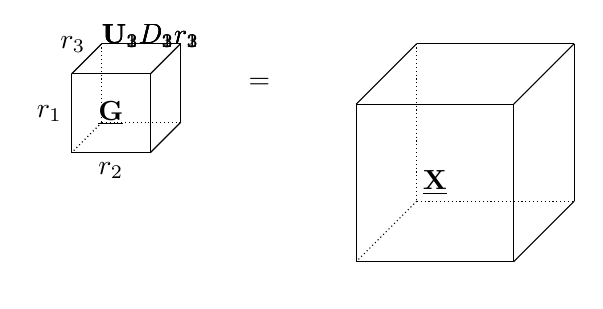
\begin{tikzpicture}[y=-1cm]
	\TensorThree{$\ten{G}$}{$r_1$}{$r_2$}{$r_3$}{1}{1}{1}
  \node at (2,0.5) {$=$};
	\begin{scope}[shift={(4,0)}]
	\TensorThree{$\ten{X}$}{}{}{}{2}{2}{2}
	\begin{scope}[shift={(-0.0707, -0.0707)}]
    \MatrixSkewed{$\mat{U}_1$}{$D_1$}{$r_1$}{1}{2}
  \end{scope}
	\begin{scope}[shift={(-0.1,0)}]
    \MatrixLeft{$\mat{U}_2$}{$D_2$}{$r_2$}{1}{2}
  \end{scope}
	\begin{scope}[shift={(0,2.1)}]
    \MatrixBelow{$\mat{U}_3$}{$D_3$}{$r_3$}{2}{1}
  \end{scope}
  \end{scope}
\end{tikzpicture}

	\caption{A visualization of the multilinear projection learnt by Higher Order
		Discriminant Analysis (\textsc{hoda}) for a dataset of $N$ second order tensors
		$\ten{X}$ of shape $(D_1,D_2)$.
		\textsc{hoda} finds projection matrices $\mat{U}_k$ such that maximal
		discriminability between classes is achieved in the projected core tensors
		$\ten{G}$ with reduced dimensionality $(r_1,r_2)$.}
	\label{fig:hoda-backward}
\end{figure}
Analogous to the \textsc{tucker} decomposition, \textsc{hoda} is a dimensionality
reduction decomposition that results in a dense core tensor $\ten{G}$, and
imposes an orthogonality constraint on $\mat{U}_k$ to ensure uniqueness.
However, while for the \textsc{tucker} decomposition the projection matrices
are chosen to minimize the reconstruction error, the projection matrices
$\mat{U}_k$ of \textsc{hoda} are optimized for maximal discriminability between
$\ten{G}(n)$ belonging corresponding classes with labels $c_n$.
This is a desirable property in a classification setting where samples are
high-dimensional tensors.

\textsc{hoda} optimizes discriminability in the Fisher sense, by optimizing the
Fisher ratio between $\phi$ the core tensors $\ten{G}(n)$
\begin{equation}
	\phi = \argmax_{\mat{U}_k}
	\frac{\sum_c^CN_c\left\lVert\bar{\ten{G}}(c)-\bar{\bar{\ten{G}}}\right\rVert_F^2}
	{\sum_n^N\left\lVert\ten{G}(n)-\bar{\ten{G}}(c_n)\right\rVert_F^2}
	\label{eq:fisher}
\end{equation}
for $C$ classes with each $N_c$ samples. $\bar{\ten{G}}(c)$ is the mean of core
tensors $\ten{G}(n)$ of class $c$, and $\bar{\bar{\ten{G}}}$ the mean of
these class mean core tensors.
Equation~\ref{eq:fisher} can be solved by the iterative algorithm in
Algorithm~\ref{alg:hoda}.
To start, $\mat{U}_k$ are initialized to orthogonal matrices, e.g. by a
Multi-Linear Singular Value Decomposition (MLSVD)~\cite{Lathauwer2000} of the input data.
At each iteration, the algorithm loops trough the modes and fixes all the
projection of all but $\mat{U}_k$ corresponding to mode $k$.
It then finds a partial core tensor $\ten{G}_{-k}=\ten{X}\mmprs{\mat{U}}{k}$
Subsequently, a new projection matrix $U_k$ can be found analogous to Linear
Discriminant Analysis by constructing the within- and between-class scatter
matrices $\mat{S}_{-k,\text{w}}$ and $\mat{S}_{-k,\text{b}}$ of
$\mat{G}_{-k,k}$ the partial core tensor unfolded towards mode $k$, and solving
the generalized eigenvalue problem
\begin{equation}
  \mat{S}_{-k,\text{b}}\mat{U}_k = \mat{\lambda}\mat{S}_{-k,\text{w}}\mat{U}_k
\end{equation}

To apply \textsc{hoda} in a classification setting, the projections $\mat{U}_k$
can first be learned on a training dataset
$\left\{\ten{X}^\text{train}(m)\right\}_m^M$ with known class labels, and
training features $\left\{\ten{G}^\text{train}(m)\right\}_m^M$ can be extracted.
Next, these training features are reshaped (vectorized) into vectors
$\left\{\vec{g}^\text{train}(m) \in \mathbb{R}^{\prod_k^Kr_k}\right\}_m^M$ and a classifier is
trained on these features and the corresponding class labels.
Finally, the learnt projections $\mat{U}_k$ can be applied to unseen testing
dataset $\left\{\ten{X}(n)^\text{test}\right\}_n^N$ and the exctracted features
$\left\{\ten{G}^\text{test}(n)\right\}_n^N$ vectorized into
$\left\{\vec{g}^\text{train}(n)\right\}_n^N$ can be
classified by the trained classifier.\todo{remove set notations for brevity}
To avoid overfitting and improve performance in low sample size settings, the
\textsc{HODA} problem can be regularized by shrinking the the partial
whithin-class scatter matrix~\cite{Phan2010} with a shrinkage factor
$\alpha_k$ at each step such that the generalized eigenvalue problem becomes
\begin{equation}
	\mat{S}_b^{(-k)}\mat{U}_k =
	\mat{\lambda}((1-\alpha_k)\mat{S}_w^{(-k)}-\alpha_k\mat{I})\mat{U}_k
\end{equation}
Like in Linear Discriminant Analysis, the shrinkage parameter $\alpha_k$ can
also be estimated in a data driven way in \textsc{hoda}~\cite{Jorajuria2022},
e.g., using the Ledoit-Wolf procedure~\cite{Ledoit2003}.


\subsection{A forward model for \textsc{hoda}}
As a prerequisite for our proposed \textsc{bttda} model, we must first find a
way to reconstruct the original data tensor $\ten{X}$ as accurately as possible
from $\ten{G}$ after dimensionality reduction.
In neuroimaging, this is referred to as a \textit{forward model}.
While a \textit{backward model} extracts latent sources or properties from the observed
data, which can be optimised for tasks like regression or classification or
informed by prior knowledge about source propagation, a \textit{forward model} is a
generative model that expresses the observed data in function of some latent
properties or sources that are given.

The \textsc{hoda} projection in Equation~\ref{eq:hoda-backward} is an example
of a backward model.
A straightforward and computationally efficient candidate for a corresponding
forward model is
\begin{equation}
	\ten{X} = \ten{G}\mmpr{\mat{A}^\intercal} + \ten{\mathbfcal{E}}
	\label{eq:hoda-forward}
\end{equation}
with \textit{activation patterns} $\mat{A}_k \in \mathbb{R}^{D_k\times r_k}$
and unkown error term $\ten{\mathbfcal{E}}$.
\begin{figure}
	\centering
	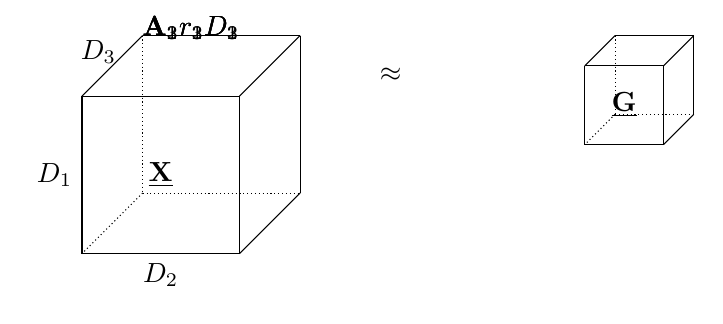
\begin{tikzpicture}[y=-1cm]
	\TensorThree{$\ten{X}$}{$D_1$}{$D_2$}{$D_3$}{2}{2}{2}
  \node at (3.15,0.5,0) {$\approx$};
	\begin{scope}[shift={(6,0)}]
	  \begin{scope}[shift={(-0.0707, -0.0707)}]
      \MatrixSkewed{$\mat{A}_1$}{$r_1$}{$D_1$}{2}{1}
    \end{scope}
	  \begin{scope}[shift={(-0.1,0)}]
      \MatrixLeft{$\mat{A}_2$}{$r_2$}{$D_2$}{2}{1}
    \end{scope}
	  \begin{scope}[shift={(0,1.1)}]
      \MatrixBelow{$\mat{A}_3$}{$r_3$}{$D_3$}{1}{2}
    \end{scope}
	    \TensorThree{$\ten{G}$}{}{}{}{1}{1}{1}
  \end{scope}
\end{tikzpicture}

	\caption{The forward projection for \textsc{hoda}. Leveraging activation
		patterns $A_k$, the original tensor $\ten{X}$ can approximately be
		reconstructed from projected core tensor of latent factors $\ten{G}$. $A_k$ are chosen such
		that the variability captured in the latent factors is maximally expressed in
		the reconstructed tensor and not in the error term.}
	\label{fig:hoda-forward}
\end{figure}

A forward model should make sure that reconstruction error is minimized and
variation captured in the latent factors is maximally captured by the forward
projection term $\ten{G}\mmpr{\mat{A}^\intercal}$, and not by the error term
$\ten{\mathbfcal{E}}$~\cite{Haufe2014}.
This gives rise to the following calculation for activation patterns
$\mat{A}_k$:
\begin{theorem}
	The activation patterns $\mat{A_k}$ for the forward model in
	Equation~\ref{eq:hoda-forward} can be calculated as
	\begin{equation}
    \mat{A}_k = \mat{\Sigma}_{\mat{X}_k}\mat{U}_k\mat{\Sigma_{X_kU}}
		\label{eq:ap}
	\end{equation}
	\label{the:ap}
\end{theorem}
With $\mat{\Sigma}_{\mat{X}_k}$ the covariance matrix of $\mat{X}_k$ tensors $\ten{X}(n)$
unfolded towards mode $k$, and $\mat{\Sigma_{X_kU}}$  the covariance matrix of
$\mat{X}_k\mat{U}$.

\subsection{Block-Term Tensor Discriminant Analysis (\textsc{bttda})}
After defining the forward model, we can construct our proposed block-term
tensor model through a deflation scheme. Assuming the core tensors $\ten{G}$
obtained by the backward projection of \textsc{hoda} does not achieve perfect
class separation, the error term $\ten{\mathbfcal{E}}$ in
Equation~\ref{eq:hoda-forward} should still contain some discriminative
information, which can be exploited to improve classifier performance.


\begin{figure*}
	\centering
	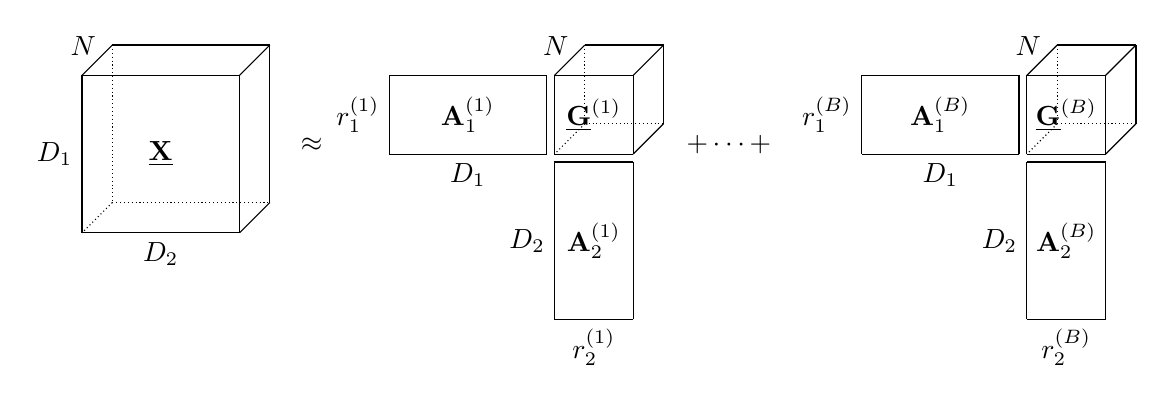
\begin{tikzpicture}[y=-1cm]
	\TensorThree{$\ten{X}$}{$D_1$}{$D_2$}{$N$}{2}{2}{1}
	\node at (3.3,.5, 2) {$\approx$};
	\begin{scope}[shift={(6,0)}]
		\TensorThree{$\ten{G}^{(1)}$}{}{}{$N$}{1}{1}{1}
	\end{scope}
	\begin{scope}[shift={(3.9,0)}]
		\TensorTwo{$\mat{A}_1^{(1)}$}{$r_1^{(1)}$}{$D_1$}{2}{1}
	\end{scope}
	\begin{scope}[shift={(6,1.1)}]
		\TensorTwo{$\mat{A}_2^{(1)}$}{$D_2$}{$r_2^{(1)}$}{1}{2}
	\end{scope}
	\node at (8.6,.5, 2) {$+\cdots+$};
	\begin{scope}[shift={(12,0)}]
		\TensorThree{$\ten{G}^{(B)}$}{}{}{$N$}{1}{1}{1}
	\end{scope}
	\begin{scope}[shift={(9.9,0)}]
		\TensorTwo{$\mat{A}_1^{(B)}$}{$r_1^{(B)}$}{$D_1$}{2}{1}
	\end{scope}
	\begin{scope}[shift={(12,1.1)}]
		\TensorTwo{$\mat{A}_2^{(B)}$}{$D_2$}{$r_2^{(B)}$}{1}{2}
	\end{scope}
\end{tikzpicture}

\end{figure*}

\subsection{Model selection}

\section{Experiments}

Decrease of MSE as f ratio increases

ERP classification
2-mode tensor
1-mode tensor

\section{Discussion}


%https://sci-hub.ru/https://ieeexplore.ieee.org/abstract/document/6287946
%https://www.sciencedirect.com/science/article/abs/pii/S0031320317301875
\printbibliography

\appendix
\section{Proof of Theorem~\ref{the:ap}}

Equations~\ref{eq:hoda-backward} and~\ref{eq:hoda-forward} can be expressed in fuction
of sample $n$ as
\begin{subequations}
	\label{eq:proj-n}
	\begin{align}
		\ten{G}(n) & = \ten{X}(n)\mmpr{\mat{U}}
		\label{eq:proj-back-n}                                                   \\
		\ten{X}(n) & = \ten{G}(n)\mmpr{\mat{A}^\intercal}+\ten{\mathbfcal{E}}(n)
		\label{eq:proj-fwd-n}
	\end{align}
\end{subequations}.
%We write Equations~\ref{eq:proj-back-n} and~\ref{eq:proj-fwd-n} respectively
%as their unfolded multi-mode products for mode $k$
%\begin{subequations}
%	\label{eq:proj-unfold}
%	\begin{align}
%		%https://www5.in.tum.de/persons/huckle/tensor-kurs_1.pdf
%		\mat{G}_k(n) & =
%		\mat{U}_n\mat{X}_n(n)\left(\mat{U}_1\otimes\mat{U}_2\otimes\cdots\otimes\mat{U}_{k-1}\otimes\mat{U}_{k+1}\otimes\cdots\otimes\mat{U}_K\right)
%		\label{eq:proj-back-unfold} \\
%		\mat{X}_k(n) & =
%		\mat{A}_n^\intercal\mat{G}_n(n)\left(\mat{A}^\intercal_1\otimes\mat{A}^\intercal_2\otimes\cdots\otimes\mat{A}^\intercal_{k-1}\otimes\mat{A}^\intercal_{k+1}\otimes\cdots\otimes\mat{A}^\intercal_K\right)
%		+ \mat{\mathbfcal{E}}_k(n)
%		\label{eq:proj-fwd-unfold}
%	\end{align}
%\end{subequations}
%According to Theorem 1 in~\cite{Haufe2014}, the activation patterns defining the
%unfolded forward model in Equation~\ref{eq:proj-fwd-unfold} corresponding to the
%unfolded backward model in Equation~\ref{eq:proj-back-unfold} is given by
%\begin{align}
%	\mat{A}_k = \mat{\Sigma}_{\mat{X}_k}\mat{U}_k
%\end{align}
Let us now express these backward and forward models in their vectorized forms:
\begin{subequations}
	\label{eq:proj-n}
	\begin{align}
		\vec{g}(n) & = \vec{x}(n)\left(\bigotimes_k^K\mat{U}_k\right)
		\label{eq:proj-back-vec}                                                  \\
		\vec{x}(n) & = \vec{g}(n)\left(\bigotimes_k^K\mat{A}_k^\intercal\right) +
		\vec{\boldsymbol\epsilon}(n)
		\label{eq:proj-fwd-vec}
	\end{align}
\end{subequations}
Since $\bigotimes_k^K\mat{U}_k$ is a Kronecker product of orthogonal matrices,
which itself is orthogonal, the activation pattern $\mat{B}$ of a forward model
corresponding to Equation~\ref{eq:proj-back-vec} is given according
to~\cite{Haufe2014} as
\begin{align*}
	\mat{B} & =
	\mat{\Sigma}_\vec{x}\left(\bigotimes_k^K\mat{U}_k\right)\mat{\Sigma}_\vec{g}^{-1} \\
	        & =
	\mat{\Sigma}_\vec{x}\left(\bigotimes_k^K\mat{U}_k\right)\left[\left(\bigotimes_k^K\mat{U}_k\right)^\intercal\mat{\Sigma_\vec{x}}\left(\bigotimes_k^K\mat{U}_k\right)\right]^{-1}
\end{align*}

Because \textsc{hoda} assumes the data covariance can be expressed as a
Kronecker product of mode-$k$ covariances
$\mat{\Sigma}_{\ten{X}_k}$\todo{citation  needed}, we get
\begin{align*}
	\mat{B} & =
	\left(\bigotimes_k^K\mat{\Sigma}_{\ten{X}_k}\right)\left(\bigotimes_k^K\mat{U}_k\right)
  \\
          & \quad \cdot \left[\left(\bigotimes_k^K\mat{U}_k\right)^\intercal\left(\bigotimes_k^K\mat{\Sigma}_{\ten{X}_k}\right)\left(\bigotimes_k^K\mat{U}_k\right)\right]^{-1}
	\\
	        &
	=\left(\bigotimes_k^K\mat{\Sigma}_{\ten{X}_k}\right)\left(\bigotimes_k^K\mat{U}_k\right)\left(\bigotimes_k^K\mat{U}_k^\intercal\mat{\Sigma}_{\ten{X}_k}\mat{U}_k\right)^{-1} \\
	        &
	=\left(\bigotimes_k^K\mat{\Sigma}_{\ten{X}_k}\right)\left(\bigotimes_k^K\mat{U}_k\right)\left[\bigotimes_k^K\left(\mat{U}_k^\intercal\mat{\Sigma}_{\ten{X}_k}\mat{U}_k\right)^{-1}\right]
	\\
	        & = \bigotimes_k^K \mat{\Sigma}_{\ten{X}_k}
	\mat{U}_k\left(\mat{U}_k^\intercal\mat{\Sigma}_{\ten{X}_k}\mat{U}_k\right)^{-1}
\end{align*}
and finally
\begin{align}
  \mat{A}_k = \mat{\Sigma}_{\ten{X}_k}
	\mat{U}_k\left(\mat{U}_k^\intercal\mat{\Sigma}_{\ten{X}_k}\mat{U}_k\right)^{-1}
\end{align}
$\blacksquare$



%Our proof follows the structure laid out in \cite{Haufe2014} (Appendix A).
%In the general case when $r_k<D_k$, $\mat{U}_k$ are not square and hence non-invertible.
%The backward and forward projections given by
%Equations~\ref{eq:hoda-backward} and~\ref{eq:hoda-forward} can be expressed in fuction
%of sample $n$ as
%\begin{equation}
%	\ten{G}(n) = \ten{X}(n)\mmpr{\mat{U}}
%	\label{eq:proj-back-n}
%\end{equation}
%and
%\begin{equation}
%	\ten{X}(n) = \ten{G}(n)\mmpr{\mat{A}^\intercal}+\ten{\mathbfcal{E}}(n)
%	\label{eq:proj-fwd-n}
%\end{equation}
%respectively, with unkown error term $\ten{\mathbfcal{E}}(n)$.
%
%Plugging the forward projection in Equation~\ref{eq:proj-fwd-n} into the backward projection in
%Equation~\ref{eq:proj-back-n} gives
%\begin{align*}
%	\ten{G}(n) & = \ten{X}(n)\mmpr{\mat{U}}                           \\
%	           & = (\ten{G}(n)\mmpr{\mat{A}^\intercal} +
%	\ten{\mathbfcal{E}}(n))\mmpr{\mat{U}}                             \\
%	           & = \ten{G}(n)\mmpr{\mat{A}^\intercal}\mmpr{\mat{U}} +
%	\ten{\mathbfcal{E}}(n)\mmpr{\mat{U}}
%\end{align*}
%Taking the tensor outer product on the left with $\ten{G}$ yields
%\begin{align*}
%	\ten{G}(n)\otimes\ten{G}(n) & = \ten{G}(n)\otimes\ten{G}(n)\mmpr{\mat{A}^\intercal}\mmpr{\mat{U}} \\
%	                            & \quad +	\ten{G}(n)\otimes\ten{\mathbfcal{E}}(n)\mmpr{\mat{U}}
%\end{align*}
%and when taking the expected value over samples
%\begin{align*}
%	 & \ev{\ten{G}(n)\otimes\ten{G}(n)}{n}                                                \\
%	 & \quad = \ev{\ten{G}(n)\otimes\ten{G}(n)\mmpr{\mat{A}^\intercal}\mmpr{\mat{U}}}{n} \\
%	 & \quad\quad + \ev{\ten{G}(n)\otimes\ten{\mathbfcal{E}}(n)\mmpr{\mat{U}}}{n}       \\
%	 & \quad = \ev{\ten{G}(n)\otimes\ten{G}(n)}{n}\mmpr{\mat{A}^\intercal}\mmpr{\mat{U}} \\
%	 & \quad\quad +  \ev{\ten{G}(n)\otimes\ten{\mathbfcal{E}}(n)}{n}\mmpr{\mat{U}}
%\end{align*}
%To find a forward projection that is corresponding to the backward projection,
%ensuring any variation explained by the projections is maximally captured in the
%activation patterns, we assume
%\begin{equation}
%	\ev{\ten{G}(n)\otimes\ten{\mathbfcal{E}}(n)}{n} = 0
%	\label{eq:uncorr}
%\end{equation}
%yielding
%\begin{align*}
%	 & \ev{\ten{G}(n)\otimes\ten{G}(n)}{n}                                                \\
%	 & \quad = \ev{\ten{G}(n)\otimes\ten{G}(n)}{n}\mmpr{\mat{A}^\intercal}\mmpr{\mat{U}}
%\end{align*}
%Since the covariance tensor of the latent tensor,
%$\ev{\ten{G}(n)\otimes\ten{G}(n)}{n}$,
%has full tensor rank due to the linear independance of columns in projection
%matrices $\mat{U}_k$, and it exists in $\mathbb{R}^{r_1\times r_1\times
%		r_2\times \ldots\times r_K\times r_1\times r_2\times \ldots\times r_K}$, its tensor inverse exists and we derive
%\begin{equation}
%	\ten{I} = \ten{I}\mmpr{\mat{A}^\intercal}\mmpr{\mat{U}}
%	\label{eq:identity}
%\end{equation}
%
%Plugging in the backward projection in Equation~\ref{eq:proj-back-n} into the
%forward projection in Equation~\ref{eq:proj-fwd-n} gives
%\begin{align*}
%	\ten{X}(n) & = \ten{G}(n)\mmpr{\mat{A^\intercal}}+\ten{\mathbfcal{E}}(n)   \\
%	           & = \ten{X}(n)\mmpr{U}\mmpr{A^\intercal}+\ten{\mathbfcal{E}}(n)
%\end{align*}
%From here, we can write $\ten{\mathbfcal{E}}(n)$ as
%\begin{align*}
%	\ten{\mathbfcal{E}}(n) & = \ten{X}(n) -	\ten{X}(n)\mmpr{\mat{U}}\mmpr{\mat{A}^\intercal} \\	                       & =	\ten{X}(n)(\ten{I}-\ten{I}\mmpr{\mat{U}}\mmpr{\mat{A}^\intercal})
%\end{align*}
%If we mutiply both sides with matrices $\mat{U}_k$, we obtain
%\begin{align*}
%	 & \ten{\mathbfcal{E}}(n)\mmpr{\mat{U}}                                                                   \\
%	 & \quad =  \ten{X}(n)(\ten{I}-\ten{I}\mmpr{\mat{U}}\mmpr{\mat{A}^\intercal})\mmpr{\mat{U}}              \\
%	 & \quad =	\ten{X}(n)(\ten{I}\mmpr{\mat{U}}-\ten{I}\mmpr{\mat{U}}\mmpr{\mat{A}^\intercal}\mmpr{\mat{U}})
%\end{align*}
%and by Equation~\ref{eq:identity}
%\begin{equation}
%	\ten{\mathbfcal{E}}(n)\mmpr{\mat{U}} =
%	\ten{X}(n)(\ten{I}\mmpr{\mat{U}}-\ten{I}\mmpr{\mat{U}})
%	= 0
%\end{equation}
%
%
%From Equations~\ref{eq:proj-fwd-n} and~\ref{eq:uncorr}
%\begin{align*}
%	\ten{\Sigma}_{\ten{X}} & =	\ten{\Sigma}_{\ten{G}}\times_{1,2,\ldots,K}\{\mat{A}^\intercal\}
%	\times_{K+1,K+2,\ldots,2K}\{\mat{A}^\intercal\}                                             \\
%	                       & \quad+ \ten{\Sigma}_{\ten{\mathbfcal{E}}}
%\end{align*}
%leading to
%\begin{align*}
%	 & \ten{\Sigma}_{\ten{X}}\mmpr{\mat{U}}\ten{\Sigma}_{\ten{G}}^{-1}                                                 \\
%	 & \quad =(\{\mat{A}^\intercal\}\times\ten{\Sigma}_{\ten{G}}\mmpr{\mat{A}^\intercal} +
%	\ten{\Sigma}_{\ten{\mathbfcal{E}}})\mmpr{\mat{U}}\ten{\Sigma}_{\ten{G}}^{-1}                                       \\
%	 & \quad=
%	\{\mat{A}^\intercal\}\times\ten{\Sigma}_{\ten{G}}\mmpr{\mat{A}^\intercal}\mmpr{\mat{U}}\ten{\Sigma}_{\ten{G}}^{-1} \\
%	 & \quad\quad + \ten{\Sigma}_{\ten{\mathbfcal{E}}}\mmpr{\mat{U}}\ten{\Sigma}_{\ten{G}}^{-1}                      \\
%	 & \quad= \{\mat{A}^\intercal\}\times\ten{\Sigma}_{\ten{G}}\ten{\Sigma}_{\ten{G}}^{-1}
%	+ \ten{\Sigma}_{\ten{\mathbfcal{E}}}\mmpr{\mat{U}}\ten{\Sigma}_{\ten{G}}^{-1}                                      \\
%	 & \quad= \ten{I}\mmpr{\mat{A}^\intercal} + 0\ten{\Sigma}_{\ten{G}}^{-1}                                          \\
%	 & \quad= \ten{I}\mmpr{\mat{A}^\intercal}
%\end{align*}

\section{P300 Paradigm benchmark datasets}
% Please add the following required packages to your document preamble:
% \usepackage{booktabs}
\begin{table}[h]
	\begin{tabular}{@{}llllllll@{}}
		\toprule
		Dataset        & \# Subjects                & \# Channels & \# Trials/class  & Trial
		length         & Sample rate                & \# Sessions & Citation                   \\ \midrule
		BI2012         & 25                         & 16          & 640 NT / 128 T   & 1s    &
		128Hz          & 2                          &                                          \\
		BI2013a        & 24                         & 16          & 3200 NT / 640 T  & 1s    &
		512Hz          & 8 for subjects 1-7 else 1  &                                          \\
		BI2014a        & 64                         & 16          & 990 NT / 198 T   & 1s    &
		512Hz          & up to 3                    &                                          \\
		BI2014b        & 38                         & 32          & 200 NT / 40 T    & 1s    &
		512Hz          & 3                          &                                          \\
		BI2015a        & 43                         & 32          & 4131 NT / 825 T  & 1s    &
		512Hz          & 3                          &                                          \\
		BI2015b        & 44                         & 32          & 2160 NT / 480 T  & 1s    &
		512Hz          & 1                          &                                          \\
		BNCI2014\_008  & 8                          & 8           & 3500 NT / 700 T  & 1s    &
		256Hz          & 1                        1                                            \\
		BNCI2014\_009  & 10                         & 16          & 1440 NT / 288 T  & 0.8s  &
		256Hz          & 3                        1                                            \\
		BNCI2015\_003  & 10                         & 8           & 1500 NT / 300 T  & 0.8s  &
		256Hz          & 1                          &                                          \\
		Cattan2019\_VR & 21                         & 16          & 600 NT / 120 T   & 1s    &
		512Hz          & 2                          &                                          \\
		EPFLP300       & 8                          & 32          & 2753 NT / 551 T  & 1s    &
		2048Hz         & 4                          &                                          \\
		Huebner2017    & 13                         & 31          & 364 NT / 112 T   & 0.9s  &
		1000Hz         & 3                          &                                          \\
		Huebner2018    & 12                         & 31          & 364 NT / 112 T   & 0.9s  &
		1000Hz         & 3                          &                                          \\
		Lee2019\_ERP   & 54                         & 62          & 6900 NT / 1380 T & 1s    &
		1000Hz         & 2                          &                                          \\
		Sosulski2019   & 13                         & 31          & 75 NT / 15 T     & 1.2s  &
		1000Hz         & 3                          &                                          \\ \bottomrule
	\end{tabular}
\end{table}
\end{document}
